\section{引言}

现代智能体并非独立运行的 LLM。它们运行在管理工具、执行环境、上下文与控制流的\emph{智能体脚手架（agent harness）}之中。脚手架因此决定了智能体如何观察环境、如何长程行动、如何从失败中恢复，是智能体能力的核心部分。典型例子包括 mini-SWE-agent~\cite{minisweagent}、OpenHands~\cite{openhands}、OpenCode~\cite{opencode}、Claude Code~\cite{claudecode}、Codex~\cite{codex} 等编程智能体脚手架，以及 OpenClaw~\cite{openclaw}、Hermes~\cite{hermes} 等通用脚手架。

早期强化学习（RL）框架，如 verl~\cite{hybridflow}、AReaL~\cite{areal} 与 slime~\cite{slime}，通常要求用户直接在训练框架内部实现智能体循环。由于现有智能体脚手架实现复杂、依赖自成体系，将其直接集成进 RL 框架十分困难。我们最初的 Agent Lightning~\cite{agentlightning} 工作提出了训练与智能体执行解耦的架构，通过 LLM 端点将任意智能体接入 RL 训练，几乎无需改动智能体本身。近来，这种基于代理的方式已被 verl Uni-Agent~\cite{uniagent}、AReaL 2.0~\cite{areal2}、slime v0.3.0~\cite{slime} 与 Polar~\cite{polar} 等框架广泛采用，自然支持在智能体脚手架上进行 RL 训练。

\add{本文将“通过部署时的同一智能体脚手架进行 RL 训练”这一范式称为\emph{\harl{}}。由脚手架——而非训练器——拥有上下文构建、工具执行与智能体-环境交互循环，训练系统则跨越服务边界观察并优化由此产生的模型调用。这种形式保留了脚手架部署时的上下文策略、工具协议与执行语义，无需在 RL 框架内部重新实现其智能体循环。}

\add{传统智能体 RL 与\harl{}都可以建模为部分可观测马尔可夫决策过程（POMDP），但二者的潜在状态与呈现给策略模型的观测不同。传统智能体 RL 中，潜在状态主要是环境状态，策略模型通过透明层几乎直接与环境交互：模型生成动作 token，环境返回观测，token 化后的观测扩展已有历史，
$p_t = \bigl(p_{t-1},a_{t-1},o_t\bigr)$。
其中 $p_t$ 为第 $t$ 步呈现给模型的 token 历史，$a_{t-1}$ 为上一步生成的动作，$o_t$ 为最新的环境观测。因此策略观察到的是连续扩展的 token 历史，一次 rollout 自然构成一条线性 token 轨迹。

在\harl{}中，策略模型不再直接与环境交互。潜在状态同时包含脚手架状态与环境状态。脚手架拥有上下文构建、控制流、工具执行与智能体编排，并为每次模型调用独立构造请求 prompt。策略只能观察到经 LLM API 送达的确切 prompt，并基于该 prompt 生成响应。因此，一次 rollout 在模型边界上呈现为一串请求-响应对，
\[
  (p_1,a_1),(p_2,a_2),\ldots,
\]
其中 $p_i$ 为第 $i$ 次 LLM 调用发送的 prompt，$a_i$ 为对应的模型响应。介于其间的脚手架与环境状态转移保持潜在。图~\ref{fig:agentic-harness-centric-comparison} 总结了这一差异。这种差异也带来了下述实现挑战——现有框架对这些挑战的不同处理方式，可能影响算法正确性与训练稳定性。}

\begin{figure*}[t]
  \centering
  \begin{minipage}[c]{0.55\textwidth}
    \centering
    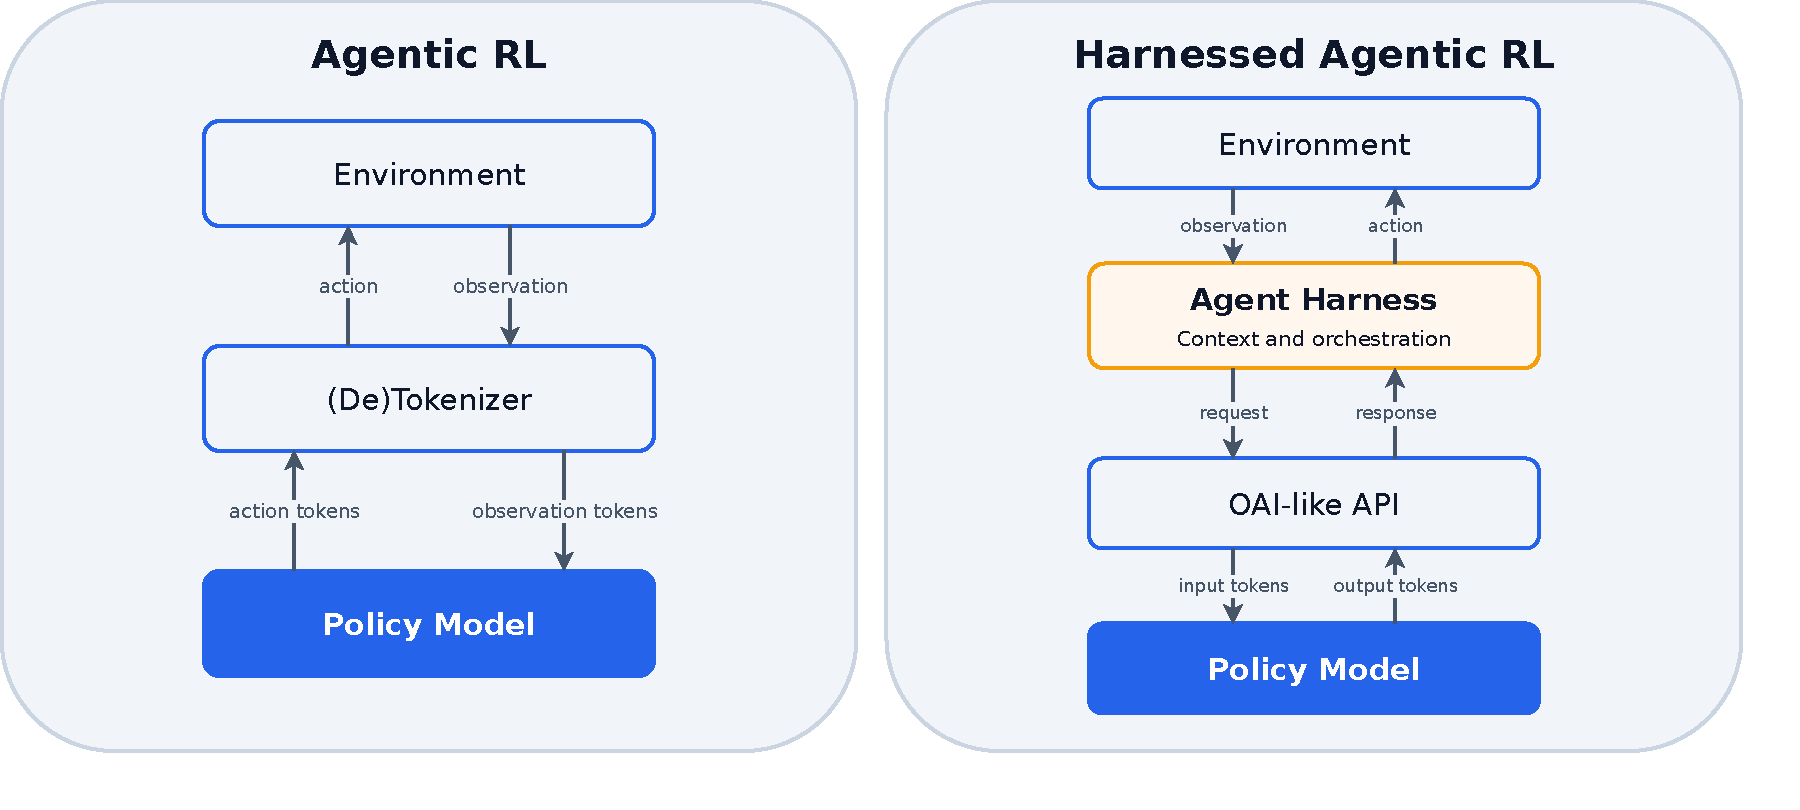
\includegraphics[width=\linewidth]
      {figures/agentic-harness-centric-comparison.pdf}
  \end{minipage}\hfill
  \begin{minipage}[c]{0.43\textwidth}
    \centering
    \scriptsize
    \setlength{\tabcolsep}{2pt}
    \renewcommand{\arraystretch}{1.06}
    \begin{tabular}{@{}
      >{\raggedright\arraybackslash}p{0.16\linewidth}
      >{\raggedright\arraybackslash}p{0.33\linewidth}
      >{\raggedright\arraybackslash}p{0.45\linewidth}@{}}
      \toprule
      & \textbf{智能体 RL} & \textbf{\add{\Harl{}}} \\
      \midrule
      \textbf{状态} &
        环境 &
        脚手架 + 环境 \\
      \hline
      \textbf{模型输入} &
        连续 token 历史 &
        每次调用独立 prompt \\
      \hline
      \textbf{智能体} &
        单一 ReAct 智能体 &
        多智能体、子智能体与交接 \\
      \bottomrule
    \end{tabular}
  \end{minipage}
  \caption{\add{传统智能体 RL 与\harl{}的对比。二者都可用 POMDP 刻画，但\harl{}在潜在执行状态中加入脚手架状态，并向策略模型暴露独立构造的模型调用 prompt。这一变化还将控制与编排移入脚手架，并使训练样本数量更加动态。}}
  \label{fig:agentic-harness-centric-comparison}
\end{figure*}

\textbf{第一个挑战是重分词与样本合并。}智能体脚手架通常通过文本消息与模型 API 通信，而 RL 训练在 token 上操作。多数框架在 $p_{i+1}$ 于 token 层面完整包含 $(p_i,a_i)$ 前缀时合并两次相邻调用。然而，重分词之后，即使文本不变，$p_{i+1}$ 中 $a_i$ 的 token ID 也可能与模型最初采样时不同。这破坏了 token 级连续性，使两次调用无法安全合并。

\textbf{第二，优势计算。}传统智能体 RL 中，每次 rollout 是一个马尔可夫过程，映射到唯一的训练样本。在\add{\harl{}}中，一次 rollout 可能产生动态数量的训练样本，原因不仅包括上述重分词问题，还包括脚手架派生子智能体、摘要压缩上下文等操作。这些动态样本给奖励与优势如何分配到训练样本带来了挑战。

\textbf{第三是损失归一化。}在\add{\harl{}}中，一次 rollout 可能映射到多个训练样本，使每个训练批次中的样本数量动态变化，损失归一化因此变得不平凡。例如，部分现有框架仍在样本层面归一化损失，使产生更多样本的 rollout 获得更大的优化权重，可能导致训练不稳定。

\textbf{第四是动态样本数量下的训练后端调度。}一批 rollout 产生的样本数量只有在脚手架执行与样本构建之后才能确定，而训练 GPU 数量及其并行配置保持固定。后端必须将变化的样本集切分为训练步与小批次，同时在固定的 GPU worker 之间均衡负载。

本文首次系统刻画了这些挑战，并进一步提出 Agent Lightning v1.0——对原始 Agent Lightning 的全面重构。它是一个面向任意智能体脚手架的轻量级 RL 训练框架。我们的设计原则是尽可能保持系统简单，仅用约 3500 行代码实现。其训练管线也内置了我们针对上述挑战的设计选择，为研究这些挑战提供了实用的试验平台。

我们使用 Agent Lightning v1.0 训练通用指令遵循智能体、搜索智能体与编程智能体。尤其地，现有智能体框架对编程智能体支持有限：缺少数据与完整训练脚本，可能源于数据清洗复杂、环境搭建困难与所需算力巨大。为填补这一空白，我们基于开源 SWE-smith 数据集与 Qwen3.5-9B~\cite{qwen35} 提供完整的数据清洗管线与可复现训练脚本。我们最终的 RL 训练仅使用 6K 训练样本与适量算力。\add{仅靠 RL，训练后的模型在 SWE-bench Verified 上从 41.8\% 提升至 56.4\%，绝对提升 14.6\%。}我们向社区发布完整工作流与脚本，以促进可复现性。
